\RequirePackage[T1]{fontenc}
\documentclass[conference,letterpaper]{IEEEtran}
\usepackage{cite}
\usepackage{amsmath,amssymb}
\usepackage{graphicx}
\usepackage{booktabs}
\usepackage{array}
\usepackage{url}
\usepackage[hidelinks]{hyperref}
\hypersetup{pdftitle={Measuring Privacy, Robustness, and Projection Tradeoffs in Federated Learning},
pdfauthor={Anurag Lnu},pdfsubject={MS Computer Science capstone report},
pdfkeywords={federated learning, differential privacy, Byzantine robustness, projection}}
\usepackage{tikz}
\usepackage{balance}
\usetikzlibrary{arrows.meta,positioning}
\hyphenation{Fed-Learn Byz-FL AUROC}
\newcommand{\R}{\mathbb{R}}
\newcommand{\clip}{\operatorname{clip}}
\newcommand{\mean}{\operatorname{mean}}
\newcommand{\gdp}{\mathrm{GDP4}}

\title{Measuring Privacy, Robustness, and Projection Tradeoffs in Federated Learning}
\author{\IEEEauthorblockN{Anurag Lnu}
\IEEEauthorblockA{MS in Computer Science\\Rochester Institute of Technology\\Rochester, New York, USA}}

\begin{document}
\maketitle

\begin{abstract}
Federated learning combines local training with server aggregation, but privacy noise, malicious uploads, and representation choice can change which aggregation policy preserves utility. This capstone implements an auditable experimental path in FedLearn and evaluates these interactions using three separately scoped studies. A frozen NIH ChestX-ray14 Effusion comparison completes 196 cells with twelve training seeds. Projection from 512 to 128 frozen features improves private-clean AUROC by 0.019176, with a paired training-seed 95\% interval of [0.011011, 0.027340], while reducing clean no-noise AUROC by 0.014923. A separate 52-cell CPU study establishes numerical agreement between Mac-only and three-host execution, but every five-round three-host pair takes longer end to end. A generated-data mechanism study completes 136 main cells and twelve qualification cells. Its private projection advantage changes sign across controlled signal-retention levels and public random bases. A padding control increases total noise energy approximately fourfold while preserving predictions, showing why parameter-noise norm alone is an insufficient utility explanation. The contribution is an inspectable engineering implementation and bounded empirical evidence. The results do not establish a novel optimizer, independent medical validation, general Byzantine robustness, or a protected end-to-end research transcript.
\end{abstract}

\begin{IEEEkeywords}
federated learning, differential privacy, Byzantine robustness, dimension reduction, reproducibility, distributed training
\end{IEEEkeywords}

\section{Introduction}
Federated learning trains a shared model from locally computed updates rather than collecting all training records at one coordinator. Iterative model averaging provides an established starting point for this setting~\cite{fedavg}. The resulting architecture, however, does not by itself determine what individual uploads reveal, whether a malicious client can corrupt training, or whether distributing a small workload reduces execution time. These questions require explicit mechanisms, trust assumptions, and measurements.

This project examines a practical decision: which combination of representation, clipping, aggregation, and privacy calibration should serve as a research baseline under a declared workload and adversary? Robust reducers such as trimmed mean have established statistical analyses~\cite{yin}, but their clean-data accuracy and behavior after calibrated privacy noise still need to be measured in the actual composite pipeline. A reducer's robustness label, lower sensitivity, or favorable interaction statistic is not sufficient evidence of useful absolute prediction performance.

The capstone therefore develops both an execution system and an experimental protocol. Its central medical workload is Effusion prediction using frozen chest-radiograph features. A later physical-host extension tests transport execution and timing without privacy or attacks. A generated-data extension then separates several explanations for projection's apparent benefit. These studies answer different questions and retain separate cohorts, budgets, and uncertainty targets.

The work makes three engineering and empirical contributions. First, it connects canonical learning components to authenticated run management, process supervision, provenance, and explicit partial outcomes. Second, it qualifies robust reducers, calibrated Gaussian perturbation, and an owned-data attacker in a source-bound research path. Third, it reports a fixed medical comparison, verified heterogeneous-host execution, and controlled projection diagnostics, including negative results. No new robust-private optimization theorem or state-of-the-art superiority claim is proposed.

The remainder follows the reporting structure used for this capstone. Section~II describes the solution and components. Section~III specifies the workload, privacy mechanism, adversary, and projection controls. Section~IV gives experimental configuration and results. Section~V discusses interpretation and validity. Section~VI compares related approaches, followed by conclusions and future work in Section~VII.

\section{Solution}
\subsection{Overview}
FedLearn exposes a browser-driven simulation path and separate source-bound batch paths. The browser path supports managed research runs through a React interface, authenticated Spring Boot API, PostgreSQL records, and a supervised Python worker. The medical batch path supports the larger controlled comparison. A separate command-line path uses the canonical gRPC coordinator and client across physical hosts. The generated projection study reuses canonical training and clipping with a study-only Gaussian coupling adapter.

Figure~\ref{fig:architecture} distinguishes these execution boundaries. The browser is not presented as a distributed-hospital scheduler. Likewise, numerical agreement across three machines does not imply that the private medical study was run as a protected distributed protocol.

\begin{figure}[t]
\centering
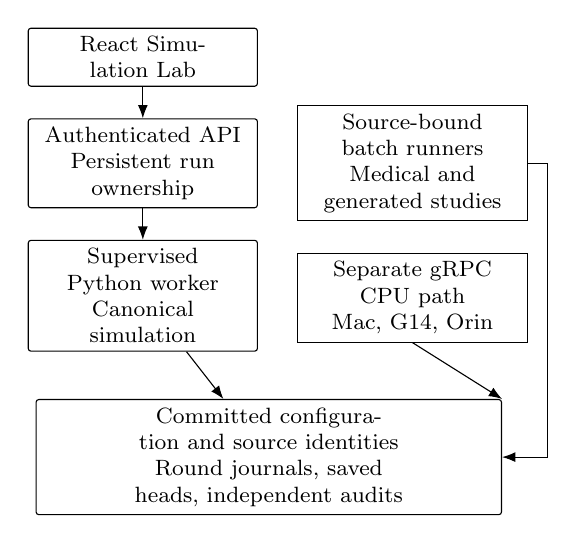
\begin{tikzpicture}[font=\footnotesize,>=Latex,
 box/.style={draw,rounded corners=1pt,align=center,text width=2.7cm,minimum height=.65cm,inner sep=3pt},
 small/.style={draw,align=center,text width=2.7cm,minimum height=.6cm,inner sep=3pt}]
\node[box] (ui) {React Simulation Lab};
\node[box,below=4mm of ui] (api) {Authenticated API\\Persistent run ownership};
\node[box,below=4mm of api] (worker) {Supervised Python worker\\Canonical simulation};
\node[small,right=5mm of api] (batch) {Source-bound batch runners\\Medical and generated studies};
\node[small,below=4mm of batch] (transport) {Separate gRPC CPU path\\Mac, G14, Orin};
\node[box,below=6mm of worker,xshift=1.6cm,text width=5.7cm] (evidence) {Committed configuration and source identities\\Round journals, saved heads, independent audits};
\draw[->] (ui)--(api);\draw[->] (api)--(worker);
\draw[->] (worker)--(evidence);
\draw[->] (batch.east)--++(.25,0)|-(evidence.east);
\draw[->] (transport.south)--(evidence.north east);
\end{tikzpicture}
\caption{Implemented execution paths. Shared components support comparable mechanisms and evidence. Browser orchestration, physical transport, and generated diagnostics remain distinct paths.}
\label{fig:architecture}
\end{figure}

\subsection{Run Management and Supervision}
The Simulation Lab resolves a canonical recipe before launch, displays completed rounds, retains run history, compares compatible terminal runs, and downloads projected research records. Authentication uses cookies and platform roles. PostgreSQL records retain run ownership. The server, rather than browser input, controls executable selection, prepared data identity, and storage locations.

The API persists a run before starting its worker and admits one active worker per application instance. The worker revalidates configuration and prepared feature integrity and writes atomic execution snapshots. Supervision enforces a deadline, drains descendants during termination, and reconciles unfinished runs on service restart using process identity. A successful progress counter alone cannot produce a completed run: the exit status, configuration, requested rounds, and qualified evidence must agree. Cancellation preserves partial outcomes. Restart reconciliation is implemented; automatic numerical continuation is not.

Browser acceptance exercised the authenticated API, database, and real Python training. Historical checks completed two three-round runs and retained a stopped run at two of twenty rounds. The later Effusion path also completed a real three-round private run and reproduced the historical A7 recipe with zero observed per-round AUROC difference and the same final digest. These are bounded execution checks, not clinical validation.

\subsection{Mechanism Composition}
The simulation driver invokes production coordinator and strategy interfaces while training logical clients sequentially inside one process. Randomness is derived from client and round identity so construction order does not silently alter another client's stream. The strategy treats uploads as deltas from the current global parameters and composes validation, clipping, reduction, Gaussian perturbation, and server state updates.

The ByzFL 0.0.11 adapter supplies established reducers through a pinned interface~\cite{byzfl}. The adapter owns update normalization, mandatory outer clipping, history semantics, and mechanism-specific sensitivity. For the private centered policy, the next center is the previously \emph{released} delta. An unnoised internal center is not carried forward. The adapter refuses unsupported private combinations, including private bucketing, median reduction, and multiple centered-clipping iterations.

The generated-data study uses the canonical local SGD trainer and clipped-mean strategy rather than a new optimizer. A reproduction-only subclass disables the parent's noise addition once and then adds explicitly coupled Gaussian draws. This supports a valid comparison between active coordinates in differently shaped heads without changing historical framework source.

\subsection{Provenance and Independent Auditing}
Prospective manifests bind the resolved design, source contents, runtime, prepared inputs, random bases, and output schema before fitting. Runners refuse an existing output directory, preserve failed cells, and stop when required qualification anchors fail. Numerical analysis reads saved heads and round evidence independently of the code that reports progress.

For medical studies, patient mappings, features, heads, and predictions remain private research artifacts. Public exports retain aggregate results and source identities. Removing local paths from an export controls disclosure but does not make the research transcript differentially private.

The generated extension records raw upload deltas, clipped aggregates, realized Gaussian draws, geometric diagnostics, final heads, and scores. Its auditor reconstructs clipping and release arithmetic, validates source and manifest bindings, checks declared noise, and independently recomputes metrics. Qualification requires completed per-cell evidence, a replaying attack check, and the independent audit. These contracts prevent an incomplete batch from being admitted merely because its summary says ``completed.''

\section{Details}
\subsection{Medical Workload and Prediction Model}
NIH ChestX-ray14 provides report-mined labels rather than prospectively adjudicated clinical ground truth~\cite{chest}. Effusion is positive when its exact label token is present; all other labels are negative. Preparation found exact RGB duplicates crossing patient or split boundaries, including conflicting labels. A conservative development quarantine removed 111 images from nine patients.

The qualified training group contains 68,650 images from 22,399 patients. Validation contains 17,763 images from 5,600 patients and was divided label-independently into a development-selection group of 9,075 images from 2,800 patients and an internal holdout of 8,688 images from 2,800 patients. The official test group contains 25,596 images from 2,797 patients. The finalist study reuses selection patients. Its remediation and extensions did not reopen holdout or official-test inputs, labels, predictions, or models.

The R0 representation is a frozen ImageNet ResNet-18~\cite{resnet} feature vector of width 512. A two-output linear head has 1,026 trainable parameters, including two biases. A fixed public orthonormal projection reduces the feature width to 128 and the trainable parameter count to 258. Training-only normalization and the prepared representation are fixed inputs to the studied mechanism. The backbone is not fine-tuned. Binary logistic-head optimization is convex in the head parameters; local minima are not an explanation for the observed policy differences.

Let $u_{i,t}$ be client $i$'s model delta at round $t$. The mandatory outer clipping rule is
\begin{equation}
\clip_C(u)=u\min\left(1,\frac{C}{\lVert u\rVert_2}\right),
\label{eq:clip}
\end{equation}
with zero mapped to zero. Uniform averaging assigns equal weight to clients, not to individual images. This choice differs from image-weighted centralized learning.

\subsection{Privacy Mechanism and Trust Boundary}
The coordinator is trusted to inspect and clip individual uploads. The abstract released update is
\begin{equation}
\widetilde{g}_t=A(\clip_C(u_{1,t}),\ldots,\clip_C(u_{N,t}))+\xi_t,
\end{equation}
where $A$ is the declared reducer and $\xi_t\sim\mathcal{N}(0,\sigma^2I)$. Adjacency replaces one honest logical client's data while preprocessing, assignment, coalition identities, and coalition data are fixed. The single-upload bound does not automatically cover replacement of a coalition member whose change can alter several malicious uploads.

For the medical comparison with $N=80$ and sixteen trimmed values per tail, the per-release sensitivity bounds are
\begin{align}
\Delta_{\mathrm{mean}}&=\frac{2C}{80}, &
\Delta_{\mathrm{trim16}}&=\frac{2C}{80-32},\\
\Delta_{\mathrm{center}}&=\frac{2\min(C,\tau)}{80}.
\label{eq:sensitivity}
\end{align}
The centered bound conditions on previously released history and one inner iteration. With $C=0.05$ and $\tau=0.0125$, the centered policy has one quarter the mean's sensitivity, while trim16 has $5/3$ the mean's sensitivity.

For $T$ full-participation Gaussian releases, Gaussian differential privacy~\cite{gdp} gives
\begin{equation}
\mu=\frac{\sqrt{T}}{z},\qquad \sigma=z\Delta.
\label{eq:gdp}
\end{equation}
The conversion used for calibration is
\begin{equation}
\delta(\epsilon;\mu)=\Phi\!\left(-\frac{\epsilon}{\mu}+\frac{\mu}{2}\right)
-e^{\epsilon}\Phi\!\left(-\frac{\epsilon}{\mu}-\frac{\mu}{2}\right),
\end{equation}
where $\Phi$ is the standard normal CDF. At $T=20$, $\epsilon=4$, and $\delta=10^{-5}$, $z\approx4.8351$. An independent normal-CDF computation checks the conversion. Medical mean noise SD is approximately 0.006044; trim16 receives $5/3$ as much coordinate noise and center\_quarter approximately 0.001511. No subsampling amplification is used.

A patient change confined to one fixed honest client is a subset of that client replacement under the same fixed-input assumptions; this gives no automatic smaller $\epsilon$. The calculation does not qualify private preprocessing, model selection, diagnostics, public research randomness, or the cumulative research transcript. It also does not provide local privacy against the coordinator or protection against a malicious host.

\subsection{Owned-Data Adversary}
The medical attacker controls sixteen persistent clients. It receives their own examples and local updates plus previously released model/history. It does not receive selection labels, current raw honest uploads, or future privacy-noise draws. The projected arm supplies the corresponding projected features and matching head; it is not attacked in the wrong feature space.

Projected gradient ascent (PGD) maximizes coalition-owned loss under an upload norm constraint. The medical recipe uses twenty steps, three restarts, step ratio 0.25, and a full-norm negative coalition-mean initialization. This gives sixty gradient and sixty-three loss evaluations per round. The surrogate forecasts benign contribution using previous releases and assumes uniform mean aggregation. It is a permitted-information heuristic rather than a reducer-specific worst-case attack. Server clipping remains mandatory after floating-point reconstruction of the malicious upload.

Oracle attacks that read current raw honest updates are retained only as separate nonprivate stress tests. Such dependence can invalidate the single-upload sensitivity premise for an honest-client data change; those attacks cannot simply inherit the same end-to-end privacy interpretation.

\subsection{Projection Controls and Noise Geometry}
The generated extension fixes a public teacher $\beta=e_0$ and draws $x\sim\mathcal{N}(0,I_{512})$ with
\begin{equation}
y\mid x\sim\operatorname{Bernoulli}\!\left(\frac{1}{1+e^{-2x_0}}\right).
\end{equation}
For $P\in\R^{512\times128}$ with $P^\top P=I$, retained teacher energy is
\begin{equation}
\eta=\lVert P^\top\beta\rVert_2^2.
\end{equation}
Controlled subspaces use first column $\sqrt{\eta}e_0+\sqrt{1-\eta}e_{128}$ and remaining columns $e_1,\ldots,e_{127}$, at $\eta\in\{0,0.25,0.75,1\}$. The full dataset and teacher stay fixed as $P$ changes. These teacher-informed subspaces are oracle diagnostic controls, not a practical basis-selection algorithm. Five separate public QR-generated bases measure variability across random subspaces without selecting the best observed one.

For a two-output head with $k$ features and two biases, independent coordinate noise satisfies
\begin{align}
\mathbb{E}\lVert\xi\rVert_2^2&=(2k+2)\sigma^2,\label{eq:energy}\\
\operatorname{Var}(\delta s\mid x)&=2\sigma^2(\lVert x\rVert_2^2+1),\label{eq:score}
\end{align}
where $s$ is the difference between the two logits. These are elementary Gaussian identities, not new theoretical results.

The padding control appends 384 exact zeros to the same 128 projected features. It trains a 512-feature head while coupling both active weight rows and biases to the 128-feature arm and drawing inactive-coordinate noise independently. Each stored-space noise law remains isotropic. Padding increases total parameter-noise energy but does not change the feature norm in~\eqref{eq:score}. With no weight decay or momentum, inactive local deltas remain zero. This checks an explanation and implementation invariant; it does not justify reduced-rank noise for an unrestricted full-feature update.

\section{Evaluation}
\subsection{Experimental Setup}
Three separately frozen measurement families are summarized in Table~\ref{tab:design}. Their sample sizes are execution budgets, not interchangeable independent replications.

\begin{table}[t]
\caption{Completed Measurement Families}
\label{tab:design}
\centering\footnotesize
\begin{tabular}{@{}p{1.02in}rrp{1.0in}@{}}
\toprule
Study & Cells & Rounds & Main variable\\\midrule
NIH finalists &196&3,920&Policy, privacy, attack\\
Physical CPU &52&320&Host placement, client count\\
Generated main &136&2,720&Signal, basis, attack effort\\
Generated qualification &12&240&Parity and admission controls\\
\bottomrule
\end{tabular}
\end{table}

\subsubsection{Medical comparison}
The main matrix crosses four policies, two noise settings, two attack settings, and twelve fresh training seeds (13001--13012), producing 192 cells plus four native anchors. The policies are mean512, projected128, trim16, and one-step released-history center\_quarter. All use eighty whole-patient IID clients, full participation, zero initialization, twenty rounds, seven local epochs, batch size 256, LR 0.03, and $C=0.05$. Projection uses public basis seed 20261025. Matching $\epsilon$ changes both the reducer and its calibrated noise; it does not hold noise amplitude fixed.

The primary endpoint is projected128 minus mean512 private-clean area under the receiver operating characteristic curve (AUROC), with a prespecified technical margin of 0.01. AUROC measures score ranking; 0.5 denotes chance ranking and does not select a clinical operating threshold. A paired Student $t$ interval across twelve training seeds conditions on the fixed evaluation cohort. A separate 2,000-draw patient-cluster bootstrap keeps the twelve fitted head pairs fixed, samples whole patients, and preserves image weighting. Neither combines training and population uncertainty or adjusts away prior selection of policies on these patients. Thirty secondary contrasts are descriptive and unadjusted for multiplicity. Average precision, Brier score, and sensitivity/specificity at probability 0.5 are retained alongside AUROC.

The finalists follow a completed diagnostic stage of 126 cells. That stage established a damaging owned-data attack, screened projection widths and centered radii, and retained negative outcomes. Its two-seed results selected the policies before final fitting; the main matrix was not retuned after its interval was observed.

\subsubsection{Physical-host CPU study}
Forty-eight five-round systems cells cross 3/6/24/80 logical clients, mean512/projected128, three paired training seeds, and Mac-only versus Mac/G14/Orin placement. Four twenty-round eighty-client anchors replay historical seed 13001. Mac coordinates and retains selection; remote hosts receive assigned training rows only. One interpreter per host shares CPU arrays while preserving independent logical-client state and RNG. At most two fits per host are active, giving up to two concurrent fits in Mac-only placement and six across three hosts; the three-client case has only three actual simultaneous fits.

The recipe retains zero heads, SGD 0.03, seven local epochs, batch 256, outer clipping 0.05, and stable logical-ID reduction order. The prospective maximum absolute parameter tolerance is $10^{-5}$. Whole-cell time includes process startup, per-cell staging, and shutdown. Steady-round time uses adjacent coordinator monotonic completion times after round one. The experiment adds resources; it does not hold total concurrency constant.

\subsubsection{Generated mechanism study}
The generator creates 4,096 training and 8,192 evaluation examples once at dataset seed 20261027. Features and labels use separately named PCG64 streams. Four training seeds (24001--24004) vary partition, minibatch, attack, and Gaussian streams without changing the dataset or basis. Twenty clients receive sixteen partitions of 205 rows and four of 204. Training uses twenty rounds, one local SGD epoch, batch 128, LR 0.03, zero initialization, and $C=0.05$.

The fixed main budget contains eight Full512 clean cells, thirty-two controlled-retention clean cells, forty random-basis clean cells, eight padded clean cells, and forty-eight attacked cells: 136 in total. Five bases (20261101--20261105) cross all four training seeds and both noise settings. The padding and attacked projected arms use basis 20261101. Attacked cells cross Full512 and Random128 with noise and 20/80/160 steps per restart, keeping three restarts. A fixed four-client coalition uses only owned data and prior releases.

GDP4 uses the same $(\epsilon,\delta)$ and twenty-release calibration but $N=20$, giving sensitivity 0.005 and noise SD approximately 0.024176. This is four times the medical mean SD because client count differs. The synthetic study is therefore not a matched medical accuracy experiment. Four training seeds and five bases support finite-grid descriptive summaries rather than discovery significance tests. Qualification is separately capped at twelve cells and thirty minutes, and main execution at twelve hours. All planned cells completed once without budget expansion or replacement fits.

\subsection{Results}
\subsubsection{Medical utility and uncertainty}
All 196 medical cells completed 3,920 full-cohort rounds. Four native/ByzFL anchors had numerically zero maximum parameter difference, without asserting bytewise equality. An independent audit reconciled 150 source files and all 31 paired-seed contrasts, with maximum contrast arithmetic difference $5.6\times10^{-17}$. Every saved head passed five-metric rescoring and independent weighted-AUROC checks.

\begin{table}[t]
\caption{NIH Effusion Finalist AUROC Means Across Twelve Training Seeds}
\label{tab:medical}
\centering\footnotesize
\begin{tabular}{@{}lrrrr@{}}\toprule
Policy & \shortstack{Clean\\no noise} & \shortstack{PGD\\no noise} & \shortstack{Clean\\GDP4} & \shortstack{PGD\\GDP4}\\\midrule
mean512 &0.807298&0.528545&0.740361&0.551304\\
projected128 &0.792375&0.761839&0.759536&0.683331\\
trim16 &0.807002&0.599442&0.678365&0.605114\\
center\_quarter &0.805107&0.722725&0.666497&0.508300\\\bottomrule
\end{tabular}
\vspace{2pt}
\begin{minipage}{\columnwidth}\footnotesize
GDP4: central update mechanism with $\epsilon=4$, $\delta=10^{-5}$ under the fixed-input honest-client replacement scope. All entries use the same development-selection patients. Means are not confidence bounds. Native anchors are excluded.
\end{minipage}
\end{table}

Table~\ref{tab:medical} and Fig.~\ref{fig:medical} report all main-arm means. Projected128's private-clean gain is $0.019176$, with paired training-seed 95\% interval $[0.011011,0.027340]$. Its SD is 0.012850, SE 0.003709, with eleven degrees of freedom. The lower endpoint exceeds the technical margin by 0.001011. The separate fixed-head patient interval is $[0.013136,0.025893]$, with 2,000 valid draws and no skipped draws.

\begin{figure}[t]\centering
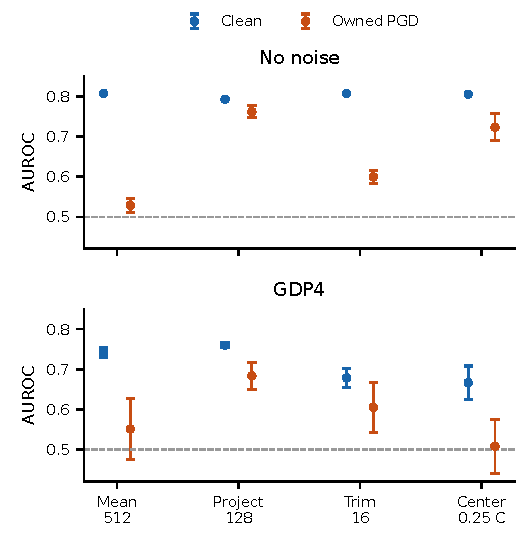
\includegraphics[width=\columnwidth]{figures/ieee-2026-10-28/medical-policies.pdf}
\caption{Medical finalist AUROC on fixed Effusion selection patients. Each point averages twelve training seeds; whiskers are one across-seed SD, not 95\% confidence intervals. The panels compare composite mechanisms under the declared noise and attack conditions.}
\label{fig:medical}\end{figure}

The two-seed pilot estimate was approximately 0.0406, more than twice the final gain. One final seed favors full width by 0.005253 and another gains only 0.000419. These retained outcomes matter when interpreting an average advantage. Selection optimism may contribute to shrinkage, but the study does not identify it as the sole cause.

\begin{figure}[t]\centering
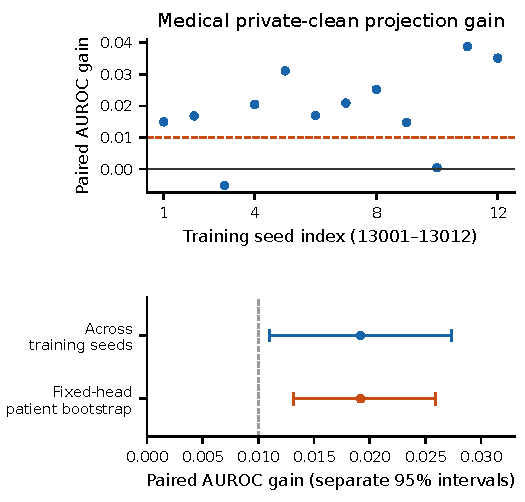
\includegraphics[width=\columnwidth]{figures/ieee-2026-10-28/medical-primary.pdf}
\caption{Individual medical private-clean projection gains and two separately conditional intervals. Dashed lines mark the 0.01 technical margin. The seed interval fixes patients; the patient-cluster interval fixes fitted head pairs. Neither is a joint or independent-cohort uncertainty statement.}
\label{fig:paired}\end{figure}

Projection reduces clean no-noise AUROC by 0.014923 while improving attacked points under this PGD. Trim16 improves private attacked utility over mean512 but loses private-clean utility. Center\_quarter performs relatively well under nonprivate attack yet has the lowest private attacked point. Lower sensitivity alone consequently does not select the most useful private policy.

The original any-finding study provides a separate caution. Its privacy-by-trimming interaction was $+0.002266150$, with paired 95\% interval $[0.000704398,0.003827901]$, but private attacked trimmed-mean AUROC was 0.618250 versus 0.627389 for the mean. A favorable interaction is not the same as a favorable absolute decision. Those historical outcomes do not replace the Effusion endpoint or cohort.

\subsubsection{Execution parity and physical-host timing}
All 52 CPU cells completed 320 rounds and 13,180 fits with acknowledged uploads. All 26 placement pairs met the prospective parameter tolerance; maximum absolute difference was $2.9802322387695312\times10^{-8}$. Mac-only anchors exactly matched their stored simulator values. Maximum three-host/historical difference was $3.725290298461914\times10^{-9}$. All final heads passed independent AUROC/loss rescoring; maximum placement AUROC discrepancy was $2.494283103393613\times10^{-7}$.

Figure~\ref{fig:cpu} summarizes paired timing ratios. Every five-round three-host pair took longer end to end: 1.866--2.931 times Mac-only time. Every three-client pair improved steady-round time, whereas every 24/80-client pair worsened it. Six-client projected128 results were mixed. This is a measured negative result for short-job placement, not a failed numerical execution.

\begin{figure}[t]\centering
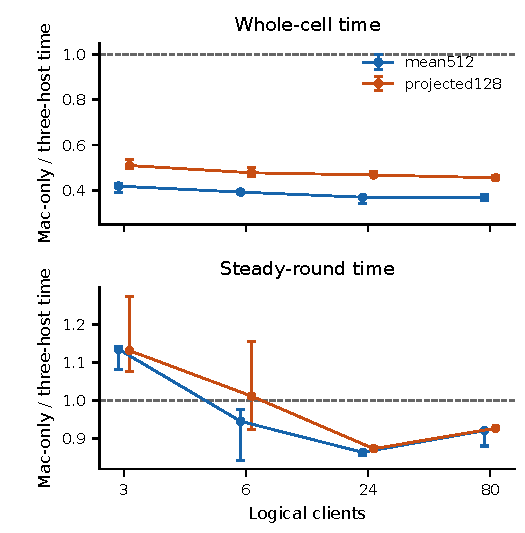
\includegraphics[width=\columnwidth]{figures/ieee-2026-10-28/cpu-placement.pdf}
\caption{Mac-only time divided by three-host time. Ratios above one favor three hosts. Markers are medians over three pairs; whiskers are observed minimum/maximum, not confidence intervals. Whole-cell and steady-round measurements have different timing boundaries.}
\label{fig:cpu}\end{figure}

The audit reconciled raw journals, fits/uploads, seven-epoch partial batches, sample counts, and evaluated aggregates, then regenerated the public analysis. Peak client-process RSS was 626.7 MiB on Mac, 413.6 MiB on G14, and 474.6 MiB on Orin; the coordinator is separate. Communication counts cover training-RPC protobuf messages and exclude registration, heartbeats, framing, and SSH. Startup, staging, polling, serialization, and background workloads were not isolated as causal bottlenecks.

\subsubsection{Controlled signal-retention boundary}
The generated main study completed 136 cells, 2,720 rounds, and 54,400 client fits, following twelve qualification cells with 240 rounds and 4,800 fits. The independent audit verified source and manifest identity, clipping, Gaussian draws, diagnostics, heads, and metrics. No main cell or seed was added after viewing outcomes.

Table~\ref{tab:retention} and Fig.~\ref{fig:retention} show the primary controlled-retention effects. Private gain changes sign between the measured $\eta=0.25$ and 0.75 points. This brackets a change on the selected grid; it does not estimate a precise continuous threshold. All four private paired effects favor $\eta=0.75$ and one, while three of four are negative at $\eta=0.25$.

\begin{table}[t]
\caption{Generated Controlled-Retention AUROC Means}
\label{tab:retention}\centering\footnotesize
\begin{tabular}{@{}lrrr@{}}\toprule
Representation & No noise & GDP4 & GDP4 gain\\\midrule
Full512 &0.817257&0.532373&0\\
128, $\eta=0$ &0.490014&0.503203&$-0.029170$\\
128, $\eta=0.25$ &0.642828&0.527375&$-0.004998$\\
128, $\eta=0.75$ &0.790752&0.587044&$+0.054671$\\
128, $\eta=1$ &0.846058&0.616847&$+0.084473$\\\bottomrule
\end{tabular}
\vspace{2pt}\parbox{\columnwidth}{\footnotesize Four training seeds on one generated evaluation draw. Gain is relative to Full512 under GDP4. Teacher-informed subspaces are diagnostic controls.}
\end{table}

\begin{figure}[t]\centering
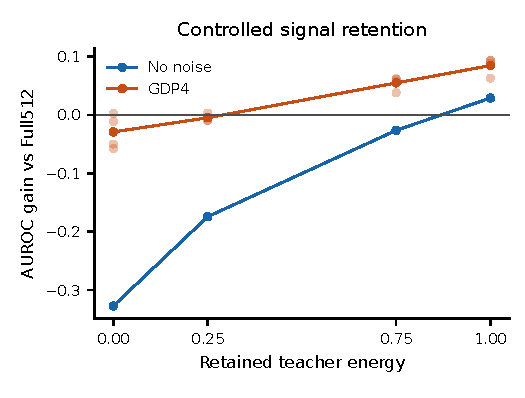
\includegraphics[width=\columnwidth]{figures/ieee-2026-10-28/signal-retention.pdf}
\caption{Generated projection gains as known teacher energy is retained. Lines connect four-seed means; faint points are individual paired effects, colored by noise setting. Lines are guides between tested settings, not an estimated boundary.}
\label{fig:retention}\end{figure}

At $\eta=0$, retained features are independent of the population label mechanism, so performance near chance is expected. At $\eta=1$, the control already gains 0.028800 without noise. Its whole private gain cannot therefore be attributed solely to Gaussian-noise reduction. The intervention fixes retained signal but still changes finite-sample learning and gradient/clipping trajectories. The known teacher score $2x_0$ attains 0.859775 AUROC against the fixed evaluation labels; it is a reference score rather than a fitted baseline or population bound.

\subsubsection{Random-basis variation and padding invariance}
Five fixed random bases produce different private gains, including a negative mean for basis 20261103 (Table~\ref{tab:bases}). Across the five private basis means, sample SD is 0.009158. Within-basis training-seed SD ranges from 0.009316 to 0.027989. These are separate finite-grid summaries, not independent variance-component estimates. The twenty points are not twenty independent projection draws.

\begin{table}[t]
\caption{Generated Random-Projection Basis Effects}
\label{tab:bases}\centering\footnotesize
\begin{tabular}{@{}rrrr@{}}\toprule
Basis & Retained $\eta$ & GDP4 AUROC & GDP4 gain\\\midrule
1 &0.276566&0.545908&$+0.013535$\\
2 &0.272852&0.539567&$+0.007194$\\
3 &0.225163&0.522270&$-0.010104$\\
4 &0.236856&0.541034&$+0.008660$\\
5 &0.239445&0.532668&$+0.000295$\\\bottomrule
\end{tabular}
\vspace{2pt}\parbox{\columnwidth}{\footnotesize Bases 1--5 correspond to public seeds 20261101--20261105. Means use four paired training seeds; gains reference private Full512. No best basis was selected.}
\end{table}

\begin{figure}[t]\centering
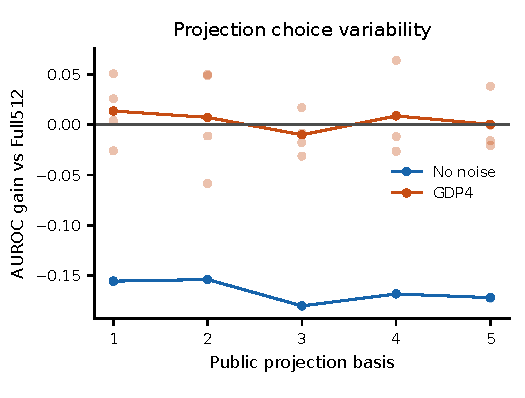
\includegraphics[width=\columnwidth]{figures/ieee-2026-10-28/random-bases.pdf}
\caption{Generated variability across public bases. Curves show means and faint points individual paired effects, colored by noise setting. The shared four Full512 baselines are reused, not counted as additional independent fits.}
\label{fig:bases}\end{figure}

This sign change establishes instability across the tested synthetic subspaces. It does not establish that the original NIH basis was lucky or quantify basis uncertainty on medical patients.

The padded head increases stored/noised parameters from 258 to 1,026. Equation~\eqref{eq:energy} predicts energy ratio $1026/258=3.976744$; the observed pooled ratio across eighty private releases per representation is 4.009877. Nevertheless, maximum padded/unpadded score discrepancy is $4.361227\times10^{-7}$, below the $10^{-5}$ tolerance, and per-round clipping decisions agree. Feature-null Gaussian coordinates change parameter energy without materially changing prediction on this path. This is why total parameter-noise energy cannot, by itself, explain utility.

\subsubsection{Attack effort and verification}
Each 20/80/160-step budget separately clears the generated Full512 no-noise damaging-control threshold: mean AUROC loss is approximately 0.11898, exceeding 0.02. Increasing effort changes the four tested arm means by less than 0.000017 (Fig.~\ref{fig:attack}). The corresponding nonprivate Full512 means are 0.698268, 0.698276, and 0.698276; projected means are 0.570864, 0.570880, and 0.570880. Private Full512 is approximately 0.51144 and projected utility approximately 0.52421.

\begin{figure}[t]\centering
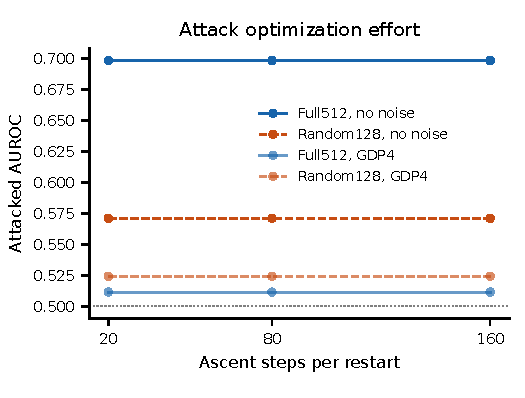
\includegraphics[width=\columnwidth]{figures/ieee-2026-10-28/attack-effort.pdf}
\caption{Generated attack-effort response. Each point averages four training seeds. A damaging no-noise Full512 control qualifies each budget separately; no monotonicity across diverging training trajectories is assumed. Saturation of this heuristic does not certify a worst-case adversary.}
\label{fig:attack}\end{figure}

At twenty steps, private projected-minus-full utility is 0.012767 under attack, compared with 0.013535 clean. The attack-adjusted difference is $-0.000768$; a special private robustness benefit does not follow from the higher attacked point. Both private attacked policies are near chance.

The generated audit's maximum errors are $1.51\times10^{-8}$ for clipped aggregates, $1.49\times10^{-8}$ for release arithmetic, $1.07\times10^{-14}$ for independent scores, $1.11\times10^{-16}$ for metrics, and $1.41\times10^{-8}$ for geometry. The runner integrates sorted ROC thresholds; the auditor uses rank sums with tie handling. Three material admission/provenance/noise-audit gaps were reproduced and corrected before qualification, not after scientific measurement.

Software verification is scoped by checkpoint. The physical-host extension's full framework gate passed 2,403 tests, with fourteen deselected and 80.23\% coverage; its runtime gate passed 802 tests. The later generated extension's bounded CPU/transport and relevant canonical-component profile passed 352 checks. The minimal environment cannot collect six legacy reproduction modules importing scikit-learn; those modules are outside that passing claim. Test totals are suite totals, not counts of newly written capstone tests.

\section{Discussion}
\subsection{What the Results Support}
Projected128 is the strongest private research candidate among the four medical policies under the frozen recipe. Its clean no-noise cost and occasional negative seed remain part of that decision. The generated controls explain why this conditional advantage cannot be generalized from stored dimension alone: lost signal can outweigh a private advantage, basis choices can change its sign, and noise in feature-null coordinates need not affect scores.

The controls add explanatory evidence rather than a new deployable defense. Knowing the synthetic teacher makes exact retention interventions possible but is unavailable in normal feature selection. The $\eta=1$ control's nonprivate gain also shows that prediction improvement can precede privacy noise. The experiments do not fully separate clipping bias, optimization trajectory, representation restriction, and finite-sample estimation into independent causal contributions.

Similarly, the centered policy's lower sensitivity does not explain its poor private utility by itself. A stale or noisy previous center is a plausible mechanism, not a result of a controlled causal ablation. Its tested failure does not refute every worker-momentum or history-based method.

The physical study establishes that numerical learning behavior can survive the transport and platform boundary within a declared tolerance. Its end-to-end slowdown is useful evidence about this short workload. It does not identify a universal hardware ordering or show that an institutional federation should be replaced with single-host training.

\subsection{Statistical and External Validity}
Repeated development-selection use is the principal medical limitation. Fresh training seeds characterize training variation on fixed patients; they do not supply new patients, independent policy confirmation, or a correction for earlier candidate selection. The seed and patient intervals target different conditional quantities and omit joint uncertainty. Secondary contrasts are descriptive and unadjusted for multiplicity.

Report-mined labels, possible undetected near-duplicates, simulated IID clients, and a frozen ImageNet representation limit transfer to clinical institutions. Label-skew pilots are not scanner, hospital, or temporal shift. The internal holdout was opened once for an earlier frozen comparison; its published aggregates remain historical and do not validate later projected policies. An external-cohort feasibility check stopped because approved access or an unused cohort was unavailable. No PhysioNet/VinDr-CXR evaluation was performed.

The generated study has one fixed dataset draw, four training seeds, five predetermined bases, linear heads, and a single owned-data attack family. Private Full512 AUROC is only 0.532373, limiting practical conclusions and creating chance-floor concerns for attack comparisons. The fixed recipe was retained rather than tuned after this weakness appeared. A basis sign change there cannot be transferred into a medical effect estimate.

\subsection{Privacy and Systems Boundaries}
The mathematical bound concerns configured update releases under fixed inputs. It does not protect every saved diagnostic, public seed, intermediate model, failure signal, or decision in the cumulative research process. Central privacy, local privacy, secure aggregation, and malicious-input validation address different trust boundaries. A trusted coordinator seeing raw updates is not equivalent to a patient-private or malicious-host-protected system.

Attacker qualification also has limits. A damaging positive control and more optimization steps do not exhaust possible strategies. Dependence on current honest uploads changes the sensitivity argument; ignoring that dependence would mix incompatible threat models. The projected attacker already sees its correct representation, so the synthetic and medical differences cannot be attributed simply to an original-space implementation error.

Three hosts remain three physical failure domains, even when eighty logical clients are multiplexed. The CPU extension does not qualify GPU execution, asynchronous training, dropout-resilient private accounting, secure transport against compromised endpoints, or hospital deployment. Actual remote disconnect/cancellation behavior has not received the same physical-host qualification as successful training. Browser and local transport checks support their specified paths, not every distributed fault scenario.

\section{Related Work}
\subsection{Robust Aggregation and History}
FedAvg provides the model-averaging foundation~\cite{fedavg}. Yin et al.~\cite{yin} analyze coordinate median and trimmed-mean distributed optimization. Their statistical guarantees motivate tested reducers but do not imply that a given clipped, noised implementation dominates under every workload. Karimireddy et al.~\cite{history} study time-coupled attacks and propose iterative clipping and worker momentum. The one-step released-history center used here is a restricted mechanism, not a reproduction of that full protocol.

Allouah et al.~\cite{trilemma} analyze privacy--robustness--utility tradeoffs and introduce SAFE-DSHB. DP-BREM and DP-BREM+~\cite{dpbrem} combine client momentum with record-level cross-silo privacy, with a separate construction for an untrusted coordinator. Those mechanisms have different privacy units and transcripts from the present honest-client replacement mechanism. They were inspected as related work, not reproduced as matched baselines. Consequently, this evaluation does not claim superiority over them.

\subsection{Privacy Calibration and Dimension Reduction}
Gaussian differential privacy supports the full-participation calibration used here~\cite{gdp}. The contribution is the declared use and independent checking of that accounting within the executed pipeline, not a new accountant.

DP-GRAPE~\cite{dpgrape} projects gradients before privatization to reduce memory costs in private deep-model training. D2P2-SGD~\cite{d2p2} combines dynamic privacy, clipping, and projection and discusses privacy, projection, and clipping errors. FedRP~\cite{fedrp} uses random projections in an ADMM-based federated protocol with different visibility assumptions. These precedents establish that projection/private optimization is an existing research direction. The present padding and teacher-retention controls are a bounded audit of an explanation for this project's results, not a first use of projected private learning.

\subsection{Frameworks and Comparison Scope}
ByzFL~\cite{byzfl} already supplies configurable aggregators, attacks, and federated benchmark utilities. This work executes its pinned reducers but remains responsible for sensitivity, clipping order, private history, attacker access, and evidence contracts.

NVIDIA FLARE documents update filters and Opacus sample-level DP training~\cite{flare}. Its PercentilePrivacy filter selectively shares weight differences; that operation alone is not the client-replacement Gaussian guarantee evaluated here. FLARE's sample-level mechanism is also not directly interchangeable with client-level calibration. No matched FLARE performance benchmark was run. Existing framework capability is therefore distinguished from experimentally demonstrated performance in this capstone.

The engineering contribution is an integrated, inspectable execution and audit path. Existing systems providing related capabilities limit novelty claims; implementation effort and test counts do not establish an original algorithm. The evaluated policies are a bounded comparison, not a comprehensive search for the best available method.

\section{Conclusion and Future Work}
The capstone implements a reproducible experimental path and measures how aggregation, privacy calibration, representation, and execution placement interact. On fixed Effusion selection patients, projected128 improves private-clean AUROC by 0.019176 at a no-noise cost of 0.014923. The three-host CPU study reproduces numerical training within tolerance but increases end-to-end time for every short-job pair. The generated extension identifies signal-retention and basis-choice limits, demonstrates prediction-preserving padding despite higher total noise energy, and records saturation of one bounded attacker.

The practical research recommendation is conditional: retain projected128 as a candidate for the declared private medical workload, preserve mean512 as the stronger clean no-noise reference, and select robust reducers using absolute clean/attacked utility rather than sensitivity or interaction alone. The empirical and engineering evidence does not establish clinical readiness, general Byzantine resilience, a novel optimizer, or production privacy.

Future work should be phased and prospective. Independent medical-cohort validation remains the strongest external-validity addition if approved access becomes available. A matched DP-BREM reproduction requires a separate privacy-unit and protocol design. Backbone or LoRA training would test model scope but adds optimization and compute confounding. A FLARE comparison needs aligned workloads and accounting; a physical failure drill needs explicit process and communication boundaries. Those extensions remain unexecuted. Any new phase should freeze its question and budget before fitting and stop if it cannot add defensible evidence within the available time.

\balance
\begin{thebibliography}{99}
\bibitem{fedavg} B. McMahan, E. Moore, D. Ramage, S. Hampson, and B. Aguera y Arcas, ``Communication-efficient learning of deep networks from decentralized data,'' in \emph{Proc. AISTATS}, vol. 54, 2017, pp. 1273--1282. [Online]. Available: \url{https://proceedings.mlr.press/v54/mcmahan17a.html}
\bibitem{yin} D. Yin, Y. Chen, K. Ramchandran, and P. Bartlett, ``Byzantine-robust distributed learning: Towards optimal statistical rates,'' in \emph{Proc. ICML}, vol. 80, 2018, pp. 5650--5659. [Online]. Available: \url{https://proceedings.mlr.press/v80/yin18a.html}
\bibitem{byzfl} M. Gonz\'alez, R. Guerraoui, R. Pinot, G. Rizk, J. Stephan, and F. Ta\"iani, ``ByzFL: Research framework for robust federated learning,'' arXiv:2505.24802, 2025. [Online]. Available: \url{https://arxiv.org/abs/2505.24802}
\bibitem{chest} X. Wang, Y. Peng, L. Lu, Z. Lu, M. Bagheri, and R. M. Summers, ``ChestX-ray8: Hospital-scale chest X-ray database and benchmarks on weakly-supervised classification and localization of common thorax diseases,'' arXiv:1705.02315v5, 2017. [Online]. Available: \url{https://arxiv.org/abs/1705.02315}
\bibitem{resnet} K. He, X. Zhang, S. Ren, and J. Sun, ``Deep residual learning for image recognition,'' in \emph{Proc. CVPR}, 2016, pp. 770--778. [Online]. Available: \url{https://openaccess.thecvf.com/content_cvpr_2016/html/He_Deep_Residual_Learning_CVPR_2016_paper.html}
\bibitem{gdp} J. Dong, A. Roth, and W. J. Su, ``Gaussian differential privacy,'' arXiv:1905.02383, 2019. [Online]. Available: \url{https://arxiv.org/abs/1905.02383}
\bibitem{history} S. P. Karimireddy, L. He, and M. Jaggi, ``Learning from history for Byzantine robust optimization,'' in \emph{Proc. ICML}, vol. 139, 2021, pp. 5311--5319. [Online]. Available: \url{https://proceedings.mlr.press/v139/karimireddy21a.html}
\bibitem{trilemma} Y. Allouah, R. Guerraoui, N. Gupta, R. Pinot, and J. Stephan, ``On the privacy-robustness-utility trilemma in distributed learning,'' in \emph{Proc. ICML}, vol. 202, 2023, pp. 569--626. [Online]. Available: \url{https://proceedings.mlr.press/v202/allouah23a.html}
\bibitem{dpbrem} X. Gu, M. Li, and L. Xiong, ``DP-BREM: Differentially-private and Byzantine-robust federated learning with client momentum,'' in \emph{Proc. USENIX Security}, 2025, pp. 3065--3082. [Online]. Available: \url{https://www.usenix.org/conference/usenixsecurity25/presentation/gu-xiaolan}
\bibitem{dpgrape} A. Mulrooney \emph{et al.}, ``Memory-efficient differentially private training with gradient random projection,'' arXiv:2506.15588v2, 2026. [Online]. Available: \url{https://arxiv.org/abs/2506.15588}
\bibitem{d2p2} Z. Jiang, M. Z. Hasan, N. Saadati, A. Balu, C. Liu, and S. Sarkar, ``Balancing utility and privacy: Dynamically private SGD with random projection,'' arXiv:2509.09485v2, 2025. [Online]. Available: \url{https://arxiv.org/abs/2509.09485}
\bibitem{fedrp} S. Najafi, M. Tavassolipour, and M. H. Narimani, ``FedRP: A communication-efficient approach for differentially private federated learning using random projection,'' arXiv:2509.10041v2, 2026. [Online]. Available: \url{https://arxiv.org/abs/2509.10041}
\bibitem{flare} NVIDIA, ``Differential privacy in FLARE,'' \emph{NVIDIA FLARE 2.9.0 Documentation}. Accessed: Oct. 28, 2026. [Online]. Available: \url{https://nvflare.readthedocs.io/en/2.9.0/user_guide/admin_guide/security/differential_privacy.html}
\end{thebibliography}
\end{document}
